\thispagestyle{timhieukhoahocnone}
\pagestyle{timhieukhoahoc}
\everymath{\color{timhieukhoahoc}}
\blfootnote{$^1$\text{\color{timhieukhoahoc}Viện Sinh thái và Môi trường Đông Dương.}}
\graphicspath{{../timhieukhoahoc/pic/}}
\begingroup
\AddToShipoutPicture*{\put(0,616){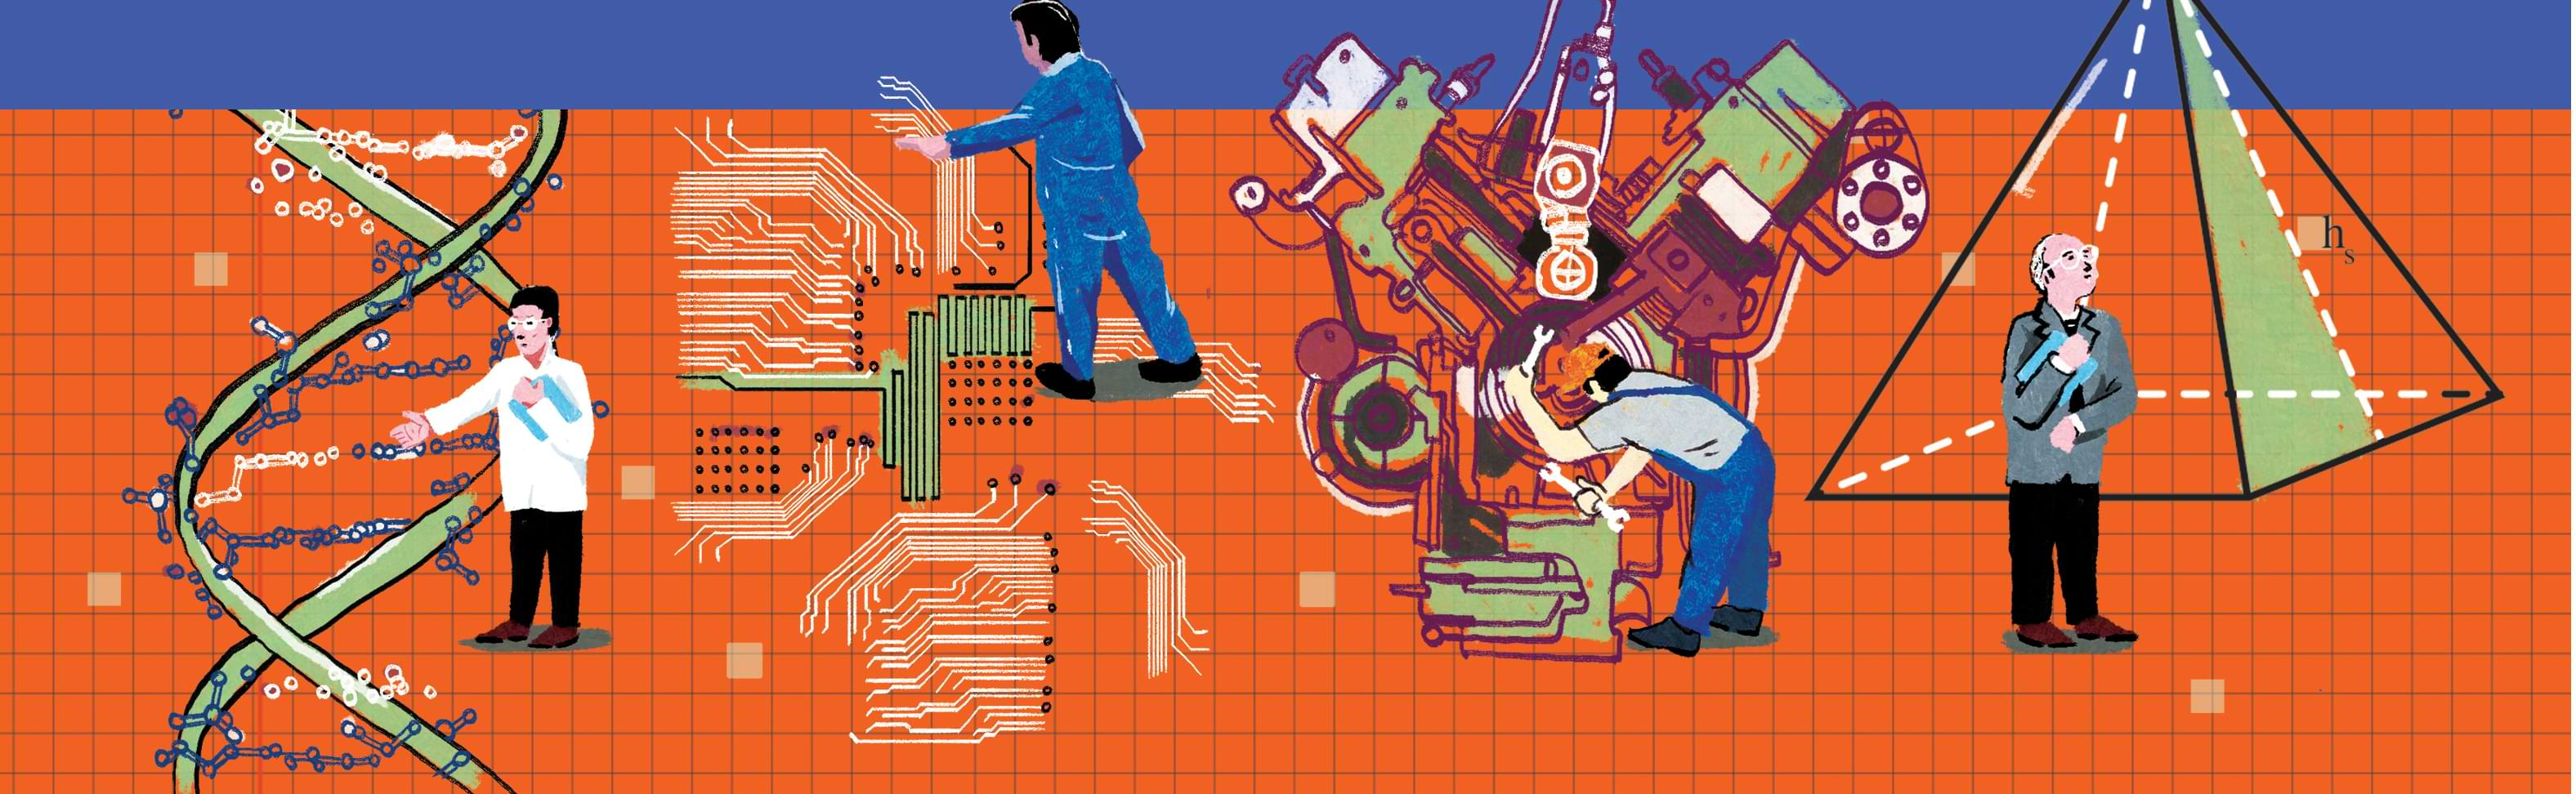
\includegraphics[width=19.3cm]{../bannertimhieu}}}
\AddToShipoutPicture*{\put(108,522){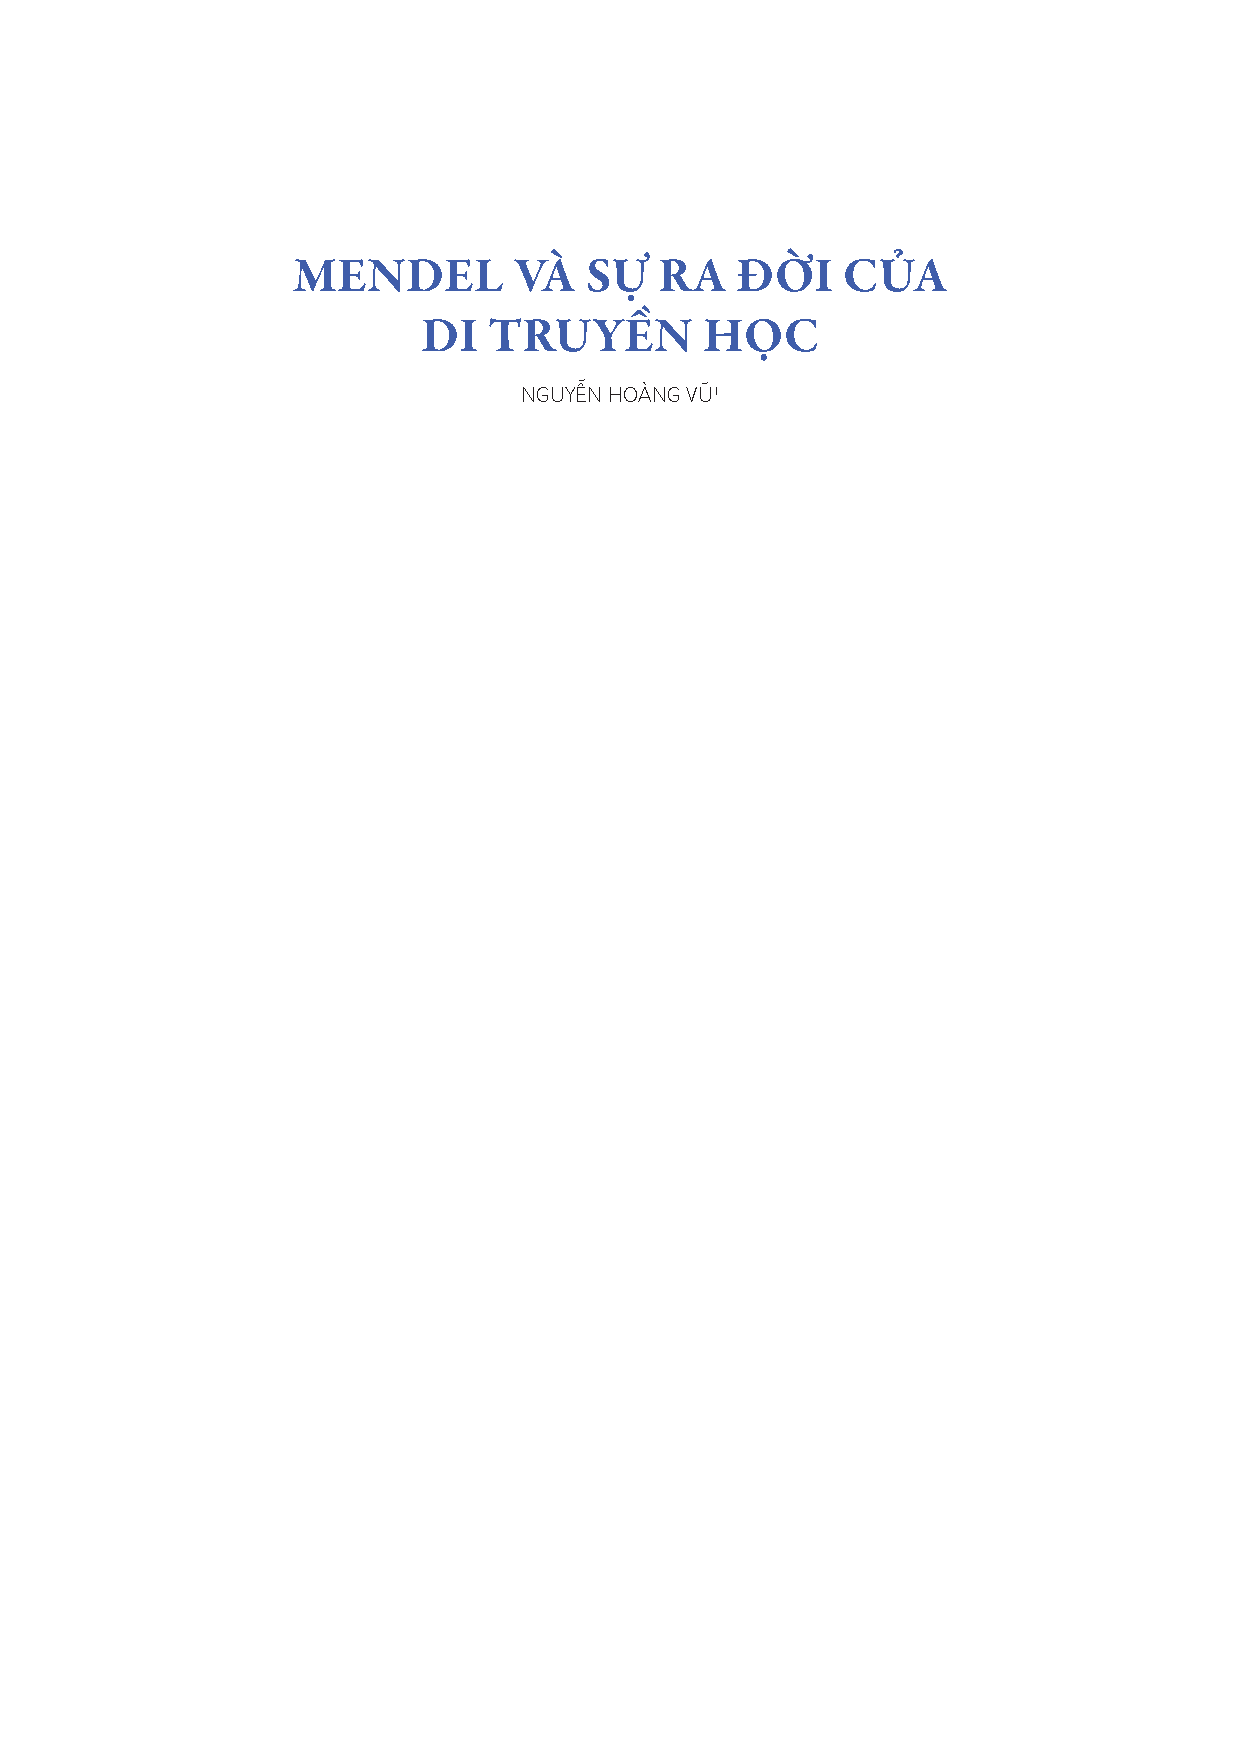
\includegraphics[scale=1]{../tieude.pdf}}}
\centering
\endgroup
\vspace*{185pt}

\begin{multicols}{2}
	Nhắc đến Mendel, người ta thường nghĩ đến các bài tập về di truyền liên quan đến tổ hợp và xác suất trong môn sinh học. Tuy nhiên, bối cảnh lịch sử cũng như sự liên hệ của các định luật Mendel với các vấn đề khác trong sinh học lại thường ít được các tài liệu chú trọng giới thiệu. Nhân dịp kỷ niệm $200$ năm ngày sinh Mendel ($20/07/1822$ -- $20/07/2022$), chúng ta hãy cùng tìm hiểu về thí nghiệm lai giống đậu kinh điển của ông, vai trò của thống kê và tổ hợp trong thí nghiệm này cùng một số vấn đề xung quanh sự ra đời của di truyền học.
	\begin{figure}[H]
		\centering
		\vspace*{-5pt}
		\captionsetup{labelformat= empty, justification=centering}
		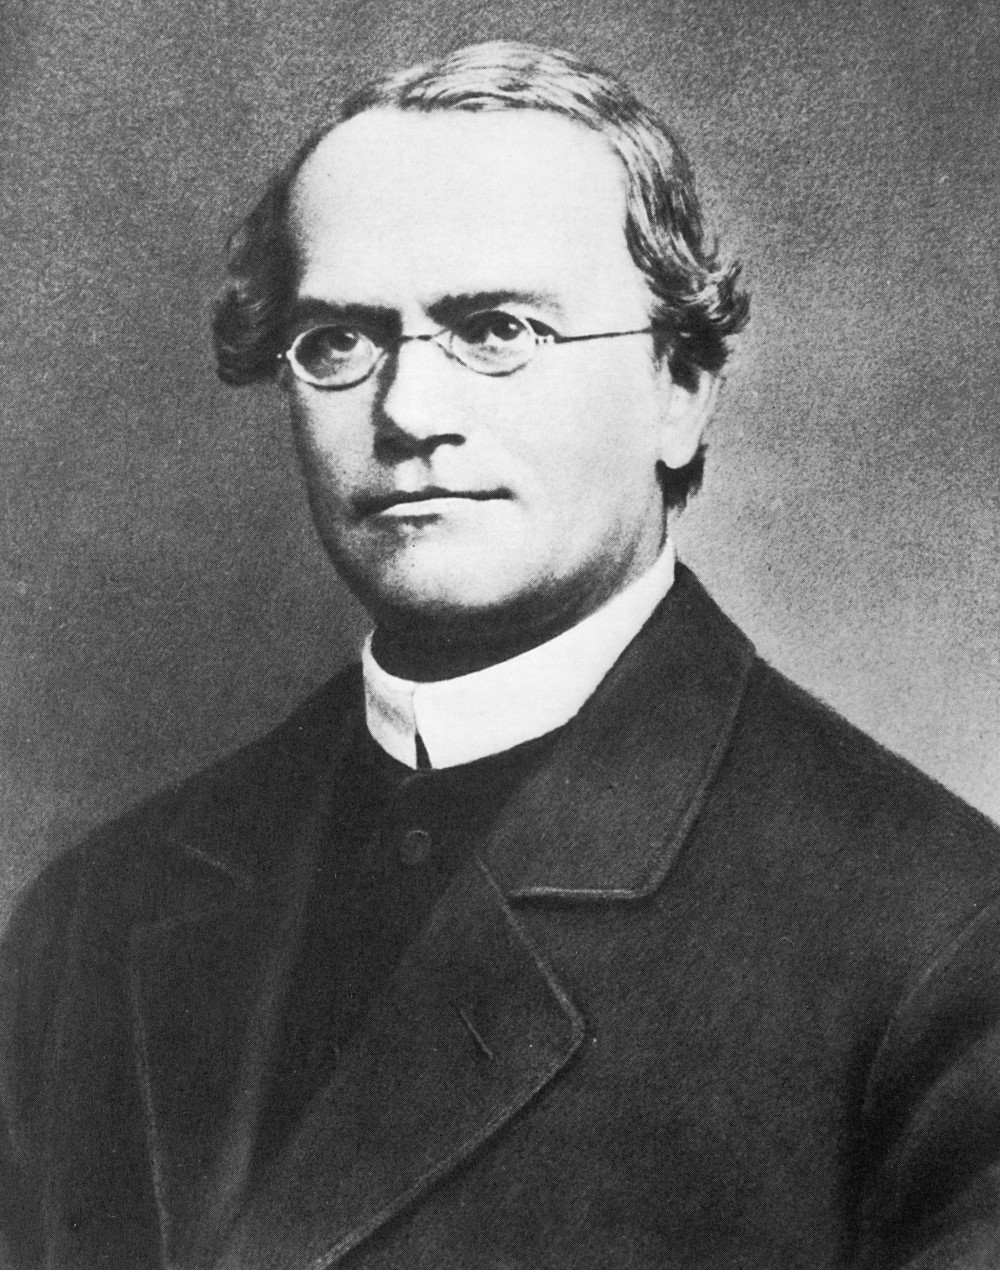
\includegraphics[width=0.76\linewidth]{image001}
		\caption{\small\textit{\color{timhieukhoahoc}Gregor Mendel ($1822$ -- $1884$).}}
		\vspace*{-5pt}
	\end{figure}
	$\pmb{1.}$ \textbf{\color{timhieukhoahoc}Giai đoạn ban đầu}
	\vskip 0.1cm
	Johann Mendel sinh năm $1822$ tại Heizendorf, vùng Silesia, thuộc đế quốc Áo (ngày nay thuộc cộng hòa Czech). Ông được gia đình cho đi học đến năm $21$ tuổi nhưng do hoàn cảnh tài chính, ông lựa chọn trở thành tu sĩ ở một tu viện ở Brno và đổi tên thành Gregor.
	\vskip 0.1cm
	Sau một thời gian, ông được tu viện phân công dạy khoa học tự nhiên tại trường học của nhà thờ ở Znojmo, một địa phương gần đó. Công việc này cũng phù hợp với sự yêu thích khoa học sẵn có của Mendel. 
	\vskip 0.1cm
	Đến năm $1849$, chính phủ Áo yêu cầu tất cả các giáo viên cần phải trải qua kỳ thi để cấp chứng chỉ hành nghề. Tuy Mendel không vượt qua được kỳ thi khảo sát do Đại học Vienna tổ chức, ông vẫn đủ tiêu chuẩn để được theo học tại đây dưới dạng sinh viên dự thính.Trong giai đoạn từ $1851$ đến $1853$, Mendel theo học nhiều môn khác nhau: vật lý, hóa học, toán học, động vật học, thực vật học và cổ sinh học. Trong quá trình đó, ông được tiếp cận với các bài giảng của Franz Unger, một nhà thực vật học nổi tiếng lúc đó. Dựa trên các nghiên cứu về hóa thạch cổ đại cùng những kiến thức mới về tế bào và sự phát triển phôi ở thực vật, Unger đưa ra một mô hình về sự tiến hóa của sinh vật: theo đó, một loài không tự nhiên sinh ra mà là hậu duệ của một loài trước đó và sự tiến hóa không tiến hành theo dạng tuyến tính mà có dạng hình cây. Unger chịu nhiều chỉ trích từ các nhân vật bảo thủ do quan điểm này ngược với các giải thích dựa trên tôn giáo. Dù bản thân là một thành viên của nhà thờ, Mendel vẫn tham gia học ở lớp của Unger.
	\vskip 0.1cm
	Tháng $8$ năm $1853$, Mendel trở lại tu viện ở Brno. Môi trường ở đây vẫn luôn chịu sự kiểm duyệt của giáo hội với các cuộc thanh tra, trong đó Mendel bị nhận định là dạng cá biệt, chuyên nghiên cứu ``các khoa học vớ vẩn". Năm $1856$, Mendel trở lại Vienna để tham dự kỳ thi sát hạch giáo viên lần thứ hai. Tuy nhiên, ông bị ốm nặng sau câu hỏi đầu tiên và phải trở về nằm giường ở Brno một thời gian. Dù mong muốn trở thành giáo viên dạy khoa học bị tan vỡ, Mendel vẫn không từ bỏ và tiến hành một thí nghiệm mà ông đã ấp ủ từ trong vài năm trước.
	\begin{figure}[H]
		\centering
		\vspace*{-5pt}
		\captionsetup{labelformat= empty, justification=centering}
		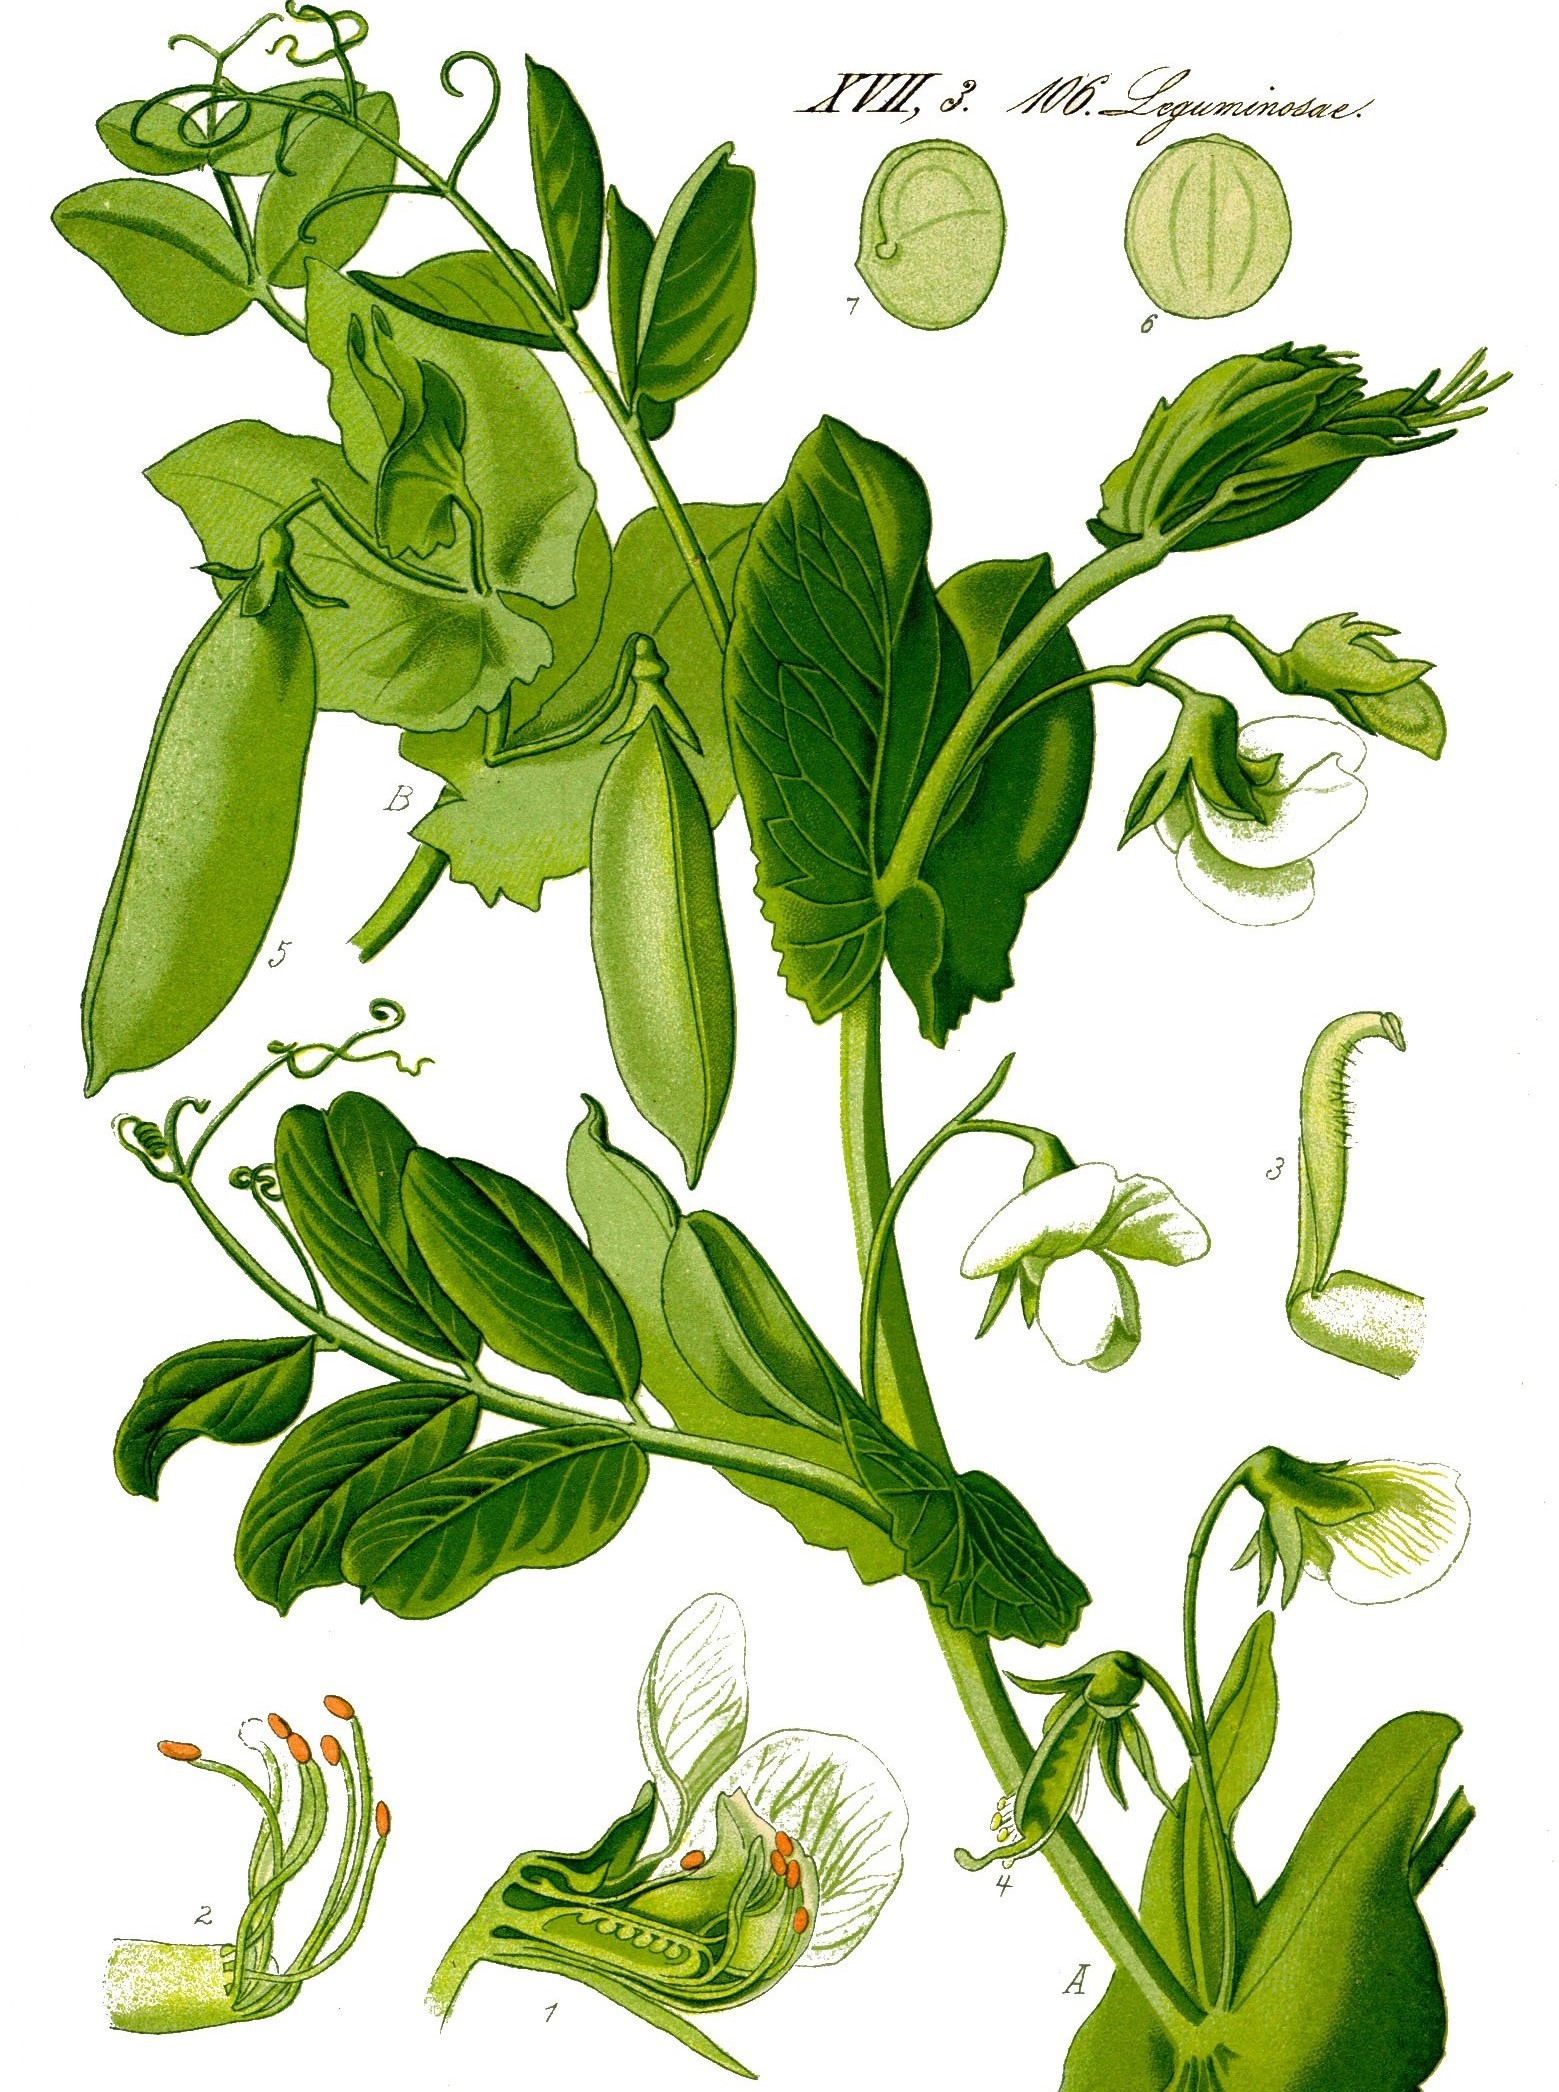
\includegraphics[width=1\linewidth]{image002}
		\caption{\small\textit{\color{timhieukhoahoc}Hình $1$. Loài đậu Pisum sativum.}}
		\vspace*{-5pt}
	\end{figure}
	Mendel tiến hành thí nghiệm để tìm hiểu các vấn đề về sự lai giống của sinh vật, một chủ đề ông được tiếp xúc trong quá trình học ở Đại học Vienna. Đối tượng của ông là loài đậu \textit{Pisum sativum}, với các dòng thuần đã được Mendel chọn lọc trong vòng hai năm trước~đó.
	\vskip 0.1cm
	$\pmb{2.}$ \textbf{\color{timhieukhoahoc}Thí nghiệm trên cây đậu}
	\vskip 0.1cm
	Quá trình thí nghiệm của Mendel được tiến hành trong suốt $8$ năm từ $1856$ đến $1863$. Trong các giống đậu đã nhân được, ông chọn ra $22$ giống để tiến hành thí nghiệm. Chúng đã được kiểm chứng là dòng thuần. Mendel sử dụng $7$ đặc điểm để phân biệt chúng, mỗi đặc điểm có hai dạng khác nhau. Các đặc điểm về hạt (màu sắc và bề mặt) có thể được quan sát trực tiếp trên các hạt đậu. Các đặc điểm còn lại yêu cầu việc gieo hạt và quan sát cây trưởng thành.
	\vskip 0.1cm
	$\pmb{2.1}$ \textbf{\color{timhieukhoahoc}Tỷ lệ trong lai giống}
	\vskip 0.1cm
	Đầu tiên, Mendel tiến hành lai các dòng thuần (F$0$) với nhau để cho ra thế hệ lai F$1$. Kết quả cho thấy với mỗi một đặc điểm, sẽ có một dạng trội mà tất cả các F$1$ đều biểu hiện theo dạng này, dạng còn lại trở thành dạng lặn. Tiếp theo, Mendel cho các F$1$ tự thụ phấn để sinh ra các F$2$. Kết quả thống kê cho thấy tỷ lệ trội~:~lặn ở F2 gần với tỷ lệ $3$~:~$1$ cho cả $7$ đặc điểm. Đặc biệt, khi cho hạt của cùng một cây F$1$ hoặc trong cùng một quả mọc lên, dạng trội và dạng lặn đều có thể xuất hiện.
	\vskip 0.1cm
	Mendel lại tiếp tục cho các cây F$2$ tự thụ phấn để cho ra thế hệ F$3$. Ông nhận thấy rằng các F$2$ mang đặc điểm lặn cho ra thế hệ F$3$ giống như vậy. Trong các cây F$2$ mang đặc điểm trội, $2/3$ trong số chúng có F$3$ theo tỷ lệ trội~:~lặn là $3$~:~$1$, giống với khi lai hai dòng thuần; còn $1/3$ còn lại cho F$3$ toàn bộ trội (các tỷ lệ này đã được làm tròn từ dữ liệu thống kê). Từ kết quả này, Mendel nhận thấy khi lai các cây lai F$1$, một nửa các hạt thu được (F$2$) sẽ là dạng lai giống như F$1$ còn một nửa còn lại trở thành dòng thuần trội hoặc dòng thuần lặn (giống F$0$) với số lượng như nhau.
	\vskip 0.1cm
	Ông tiến hành lặp lại các thí nghiệm trên các đặc điểm của hạt đậu cho $6$ thế hệ và trên các đặc điểm của cây đậu cho $4$ thế hệ liên tiếp. Kết quả cho cả $7$ đặc điểm khẳng định rằng thế hệ sau của các cây lai từ hai dòng thuần được phân chia theo tỷ lệ $2$~:~$1$~:~$1$ cho dạng lai và hai dạng thuần.
	\vskip 0.1cm
	Mendel ký hiệu $A$ là dạng trội, $a$ là dạng lặn và $Aa$ là dạng lai kết hợp của hai dạng thuần (Tất nhiên là lúc đó Mendel không thể biết được việc vật liệu di truyền có hai bản sao theo cặp. Theo cách ký hiệu ngày nay, các ký hiệu trên phải là $AA$, $aa$ và $Aa$). Ông biểu diễn thế hệ F$2$ theo biểu thức: $A + 2Aa + a$.
	\begin{figure}[H]
		\centering
		\vspace*{-5pt}
		\captionsetup{labelformat= empty, justification=centering}
		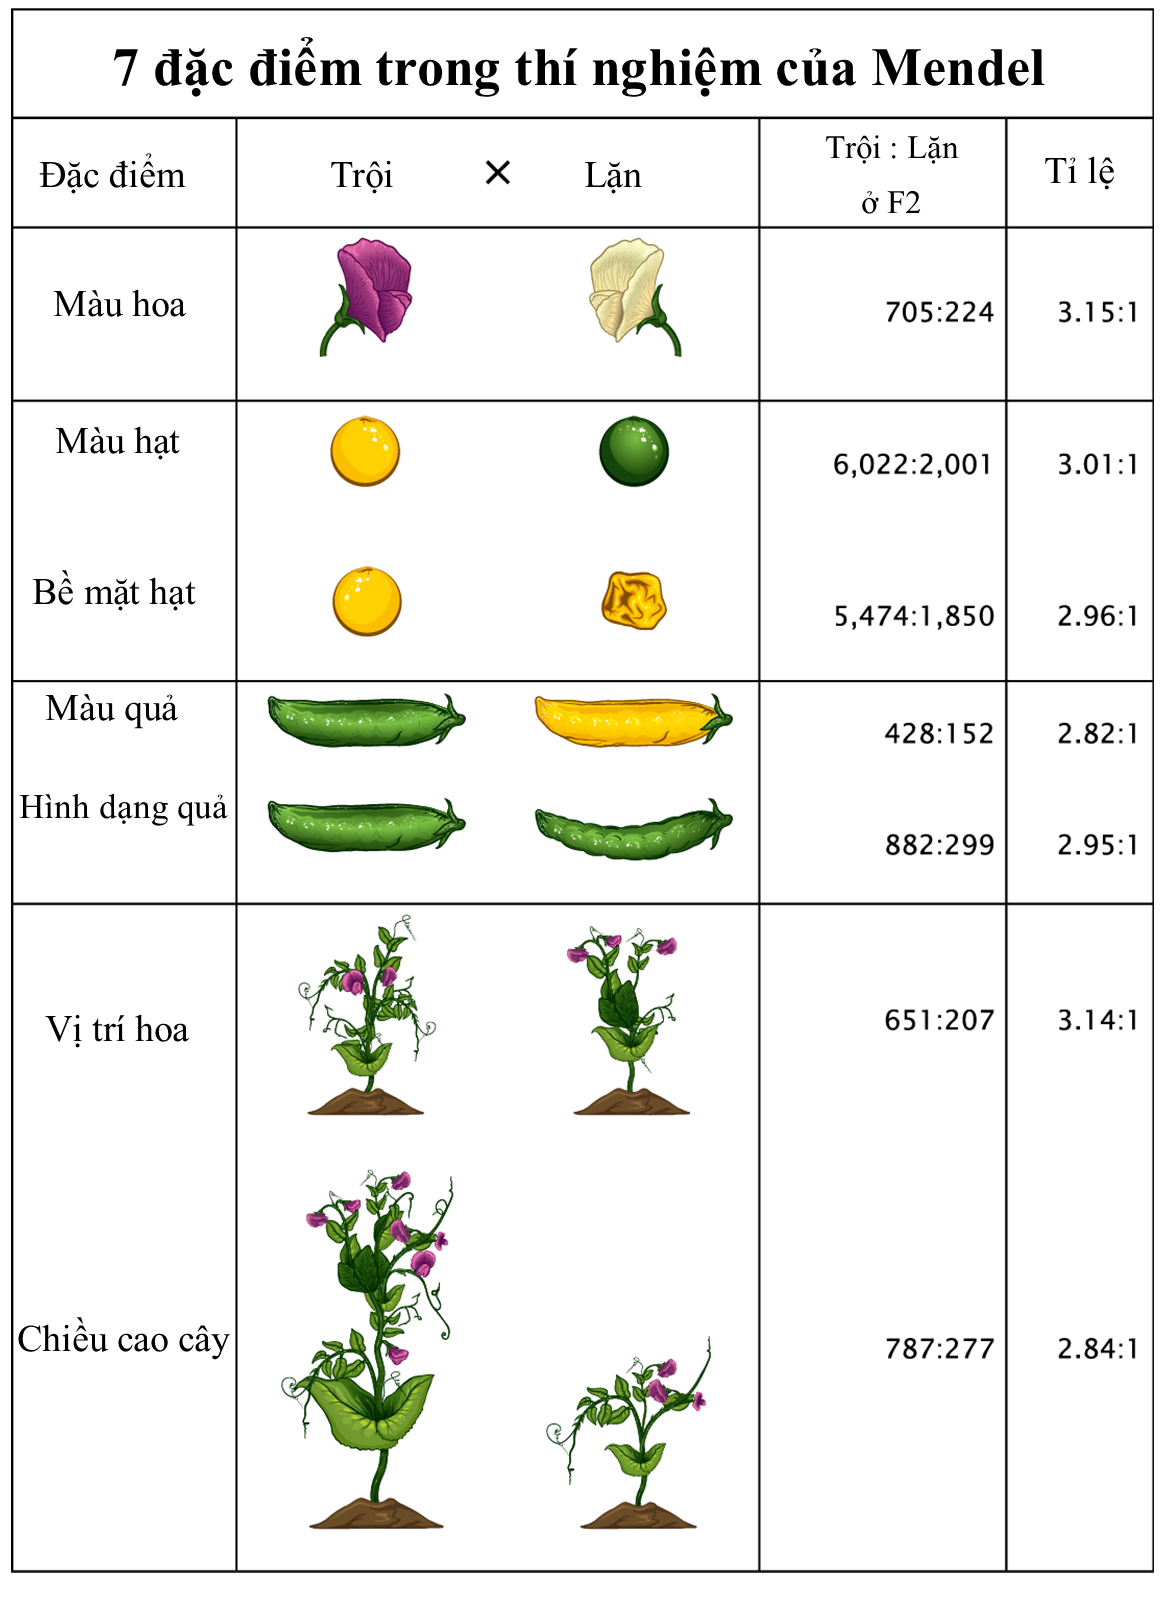
\includegraphics[width=1\linewidth]{image003}
		\caption{\small\textit{\color{timhieukhoahoc}Hình $2$. Các đặc điểm Mendel nghiên cứu trong thí nghiệm lai cùng tỷ lệ trội~:~lặn quan sát được.}}
		\vspace*{-10pt}
	\end{figure}
	$\pmb{2.2}$ \textbf{\color{timhieukhoahoc}Lai nhiều đặc điểm}
	\vskip 0.1cm
	Mendel lại tiếp tục tiến hành thí nghiệm về sự tương tác giữa nhiều hơn một đặc điểm khác nhau khi lai. Trong thí nghiệm cho hai đặc điểm, Mendel lai dòng thuần hạt tròn $(A)$ -- hạt vàng $(B)$ với dòng thuần hạt nhăn $(a)$ -- hạt xanh $(b)$. Ở đây, các chữ cái in biểu diễn dạng trội còn các chữ cái thường biểu diễn dạng lặn của một đặc điểm. Kết quả cho F$1$ toàn bộ có hạt tròn và vàng. Khi cho $15$ cây F$1$ tự thụ phấn, Mendel thu được $556$ hạt F$2$. Các F$2$ này được trồng thành cây và đặc điểm của các hạt của chúng (tức F$3$) được thống kê để phân loại F$2$.
	\begin{table}[H]
		\vspace*{-5pt}
		\centering
		\captionsetup{labelformat= empty, justification=centering}
		\resizebox{\columnwidth}{!}{\begin{tabular}{|l|p{1.6cm}|p{2cm}|p{1.6cm}|}
				\hline
				&$A$&	$Aa$&	$A$\\
				\hline
				$B$&	$AB$ (tròn vàng)~:~$38$&	$AaB$ (tròn vàng + nhăn vàng)~:~$60$&	$aB$ (nhăn vàng)~:~$28$\\
				\hline
				$Bb$&	$ABb$ (tròn vàng + tròn xanh)~:~$65$&	$AaBb$ (tròn vàng + tròn xanh + nhăn vàng + nhăn xanh)~:~$138$&	$aBb$ (nhăn vàng và nhăn xanh)~:~$68$\\
				\hline
				$b$&	$Ab$ (tròn xanh)~:~$35$& $Aab$ (tròn xanh + nhăn xanh)~:~$67$&	$ab$ (nhăn xanh)~:~$30$\\
				\hline
		\end{tabular}}
		\caption{\small\textit{\color{timhieukhoahoc}Bảng $1$. Kết quả phân loại $556$ cây F$2$ dựa trên hạt của chúng.}}
		\vspace*{-10pt}
	\end{table}
	Mendel phân loại các dạng thu được thành ba nhóm: nhóm có cả hai đặc điểm đều là thuần ($AB$, $Ab$, $aB$ và $ab$), nhóm có một đặc điểm thuần và một đặc điểm lai ($ABb$, $aBb$, $AaB$, $Aab$) và nhóm có cả hai đặc điểm là lai ($AaBb$). Ông nhận định rằng số liệu của các dạng này: $32$, $65$, $138$ gần với bộ số $33$, $66$, $132$ ứng với tỷ lệ $1 : 2 : 4$. Có thể thấy trực giác phân tích số liệu của Mendel rất tốt. Ông kết luận rằng hiện tượng quan sát được là do sự kết hợp của hai biểu thức $A + 2Aa + a$ và $B + 2Bb +b$. Thật vậy, tiến hành phép nhân hai biểu thức này, ta được:
	\begin{align*}
		&AB + 2AaB + aB + 2ABb +4AaBb\\
		&+ 2aBb + Ab + 2Aab + ab
	\end{align*}
	Tương tự, khi tiến hành thí nghiệm lai cho ba đặc điểm, kết quả phân bố cũng phù hợp với tích của ba biểu thức $A + 2Aa + a$, $B + 2Bb +b$ và $C + 2Cc + c$.
	\vskip 0.1cm
	Một điểm tương đối thú vị ở đây là Mendel không sử dụng công thức nhân xác suất như ngày nay ta vẫn dùng khi giải các bài toán tổ hợp trong di truyền mà biểu diễn số lượng các nhóm trong mỗi đặc điểm theo biểu thức đại số với các hệ số có tỷ lệ ứng với số lượng từng nhóm rồi tiến hành nhân các biểu thức đại số để cho ra tỷ lệ giữa các nhóm tổ hợp.
	\vskip 0.1cm
	Các kết quả của hai thí nghiệm này (cũng như nhiều thí nghiệm tương tự cho các bộ đặc điểm khác) cho phép Mendel kết luận rằng việc di truyền các đặc điểm mà ông nghiên cứu là độc lập.
	\vskip 0.1cm
	$\pmb{2.3}$ \textbf{\color{timhieukhoahoc}Thí nghiệm về tế bào sinh sản}
	\vskip 0.1cm
	Trong các thí nghiệm trước, khi tiến hành lai các F$0$, Mendel đem phấn từ các cây dòng thuần lặn đến thụ phấn cho hoa của các cây dòng thuần trội. Câu hỏi đặt ra là nếu vai trò hoa/phấn hoa được đảo lại thì kết quả có vẫn luôn vậy không? Ông giả định rằng số loại tế bào noãn/phấn hoa được tạo ra bằng với số lượng các dạng tổ hợp của các dòng thuần (ví dụ $AB$, $Ab$, $aB$, $ab$ cho trường hợp hai đặc điểm). Đồng thời khi kết hợp giả định này với việc tỷ lệ của mỗi tổ hợp so với tổng số là giống nhau, Mendel hy vọng nó có thể giải thích các kết quả về phân bố tổ hợp của các đặc điểm ở những thí nghiệm trước đó.
	\vskip 0.1cm
	Đầu tiên Mendel thụ phấn cho hoa của F$0$ trội $AB$ bằng phấn từ cây F$0$ lặn $ab$ để thu được dạng lai $AaBb$. Tiếp đó, ông tiến hành $4$ quá trình thụ phấn:
	\vskip 0.1cm
	$\bullet$ cho hoa của dạng lai từ phấn hoa của $AB$
	\vskip 0.1cm
	$\bullet$ cho hoa của dạng lai từ phấn hoa của $ab$
	\vskip 0.1cm
	$\bullet$ cho hoa của $AB$ từ phấn hoa của dạng lai
	\vskip 0.1cm
	$\bullet$ cho hoa của ab từ phấn hoa của dạng lai
	\vskip 0.1cm
	Với mỗi thí nghiệm, tất cả hoa của một cây đều được thụ phấn. Mendel nhận định rằng nếu giả định của mình là đúng thì các cây lai sẽ có các tế bào noãn và tế bào phấn hoa của các dạng $AB$, $Ab$, $aB$, và $ab$. Khi chúng kết hợp với các tế bào noãn và tế bào phấn hoa từ các cây bố mẹ $AB$ và $ab$ thì sẽ có các mẫu lần lượt như sau trong từng trường hợp:
	\vskip 0.1cm
	$\bullet$ $AB$, $ABb$, $AaB$, $AaBb$
	\vskip 0.1cm
	$\bullet$ $AaBb$, $Aab$, $aBb$, $ab$
	\vskip 0.1cm
	$\bullet$ $AB$, $ABb$, $AaB$, $AaBb$
	\vskip 0.1cm
	$\bullet$ $AaBb$, $Aab$, $aBb$, $ab$
	\vskip 0.1cm
	và trong mỗi trường hợp, các dạng đều xuất hiện với tần số như nhau.
	\vskip 0.1cm
	Mendel nhận thấy kết quả thí nghiệm không phụ thuộc vào việc phấn hoa được lấy từ dòng thuần nào khi tiến hành lai F$0$. Tất nhiên, ông cũng chỉ ra rằng số liệu thống kê từ thí nghiệm không thể hoàn toàn khớp một cách chính xác như công thức toán học.
	\vskip 0.1cm
	Tiếp theo Mendel tiến hành lai một cách phức tạp hơn. Đầu tiên, ông dùng phấn hoa của $ab$ để thụ phấn cho $Ab$ để tạo dạng lai $Aab$ (ký hiệu $A$~:~hoa vàng, $a$~:~hoa trắng; $B$~:~thân dài, $b$~:~thân ngắn). Đồng thời, ông cũng dùng phấn hoa này của $ab$ để thụ phấn cho $aB$ cho ra dạng lai $aBb$. Sau đó, phấn hoa của $aBb$ được dùng để thụ phấn cho $Aab$ để cho ra các tổ hợp $AaBb$, $aBb$, $Aab$ và $ab$. Sau khi gieo hạt và quan sát, tỷ lệ $Aa$~:~$a$ và $Bb$~:~$b$ đều gần với $1$~:~$1$.
	\vskip 0.1cm
	Các kết quả trên cùng những thí nghiệm tương tự với các đặc điểm khác cho Mendel kết luận rằng ở tế bào noãn hay tế bào phấn hoa của cây lai thì tỷ lệ cho mỗi tổ hợp từ các dạng thuần là như nhau. Chẳng hạn, cây lai $AaB$ sẽ có số lượng các tế bào sinh sản với tỷ lệ $AB$~:~$aB$ gần với $1$~:~$1$. Còn cây lai $AaBb$ sẽ có tỷ lệ $AB$~:~$Ab$~:~$aB$~:~$Bb$ gần với $1$~:~$1$~:~$1$~:~$1$.
	\vskip 0.1cm
	$\pmb{3.}$ \textbf{\color{timhieukhoahoc}Sự ra đời của di truyền học}
	\vskip 0.1cm
	Mendel trình bày kết quả thí nghiệm trong suốt $8$ năm của mình ở Hội lịch sử tự nhiên Brno vào năm $1865$ và công bố bài báo về nghiên cứu này vào năm $1866$. Tuy nhiên, nó hầu như không được chú ý đến cho đến tận vài thập kỷ sau.
	\vskip 0.1cm
	Về mặt lịch sử, trong giai đoạn nửa cuối thế kỷ $19$, bản chất của sự tiến hóa của sinh vật trở thành một vấn đề nổi bật. Darwin trong cuốn sách ``Nguồn gốc các loài" năm $1859$ đề xuất thuyết tiến hóa của mình mà theo đó sự tiến hóa là một quá trình liên tục thông qua chọn lọc tự nhiên: các cá thể với các tính trạng thích nghi với điều kiện môi trường sẽ có lợi thế hơn để sống sót và sinh sản, chúng di truyền lại các tính trạng này cho hậu duệ và theo thời gian các tính trạng có ưu thế sẽ phổ biến hơn trong quần thể. Theo Darwin, quá trình này có thể dẫn đến sự tạo thành loài mới khi các quần thể của cùng một loài thích nghi với các điều kiện sống khác nhau dẫn tới sự phân hóa.
	\vskip 0.1cm
	Đồng thời, Darwin cũng đưa ra giả thuyết của mình về di truyền. Theo đó, các tế bào trong cơ thể của sinh vật sẽ sinh ra các thành phần gọi là ``gemmule". Chúng sẽ tích tụ trong tế bào sinh sản và do đó được truyền cho thế hệ sau. Việc lai giống dẫn đến sự trộn lẫn gemmule. Có những dạng gemmule sẽ trội hơn, lấn át các dạng khác. Cường độ của các dạng gemmule có thể thay đổi theo từng thế hệ và có những trường hợp biểu hiện ra các gemmule dạng lặn. Giả thuyết này được Darwin đặt tên là pangenesis.
	\vskip 0.1cm
	Francis Galton, người em họ của Darwin lại có một ý tưởng khác về tiến hóa. Galton là một nhà toán học có vai trò quan trọng trong lịch sử thống kê với việc định nghĩa các khái niệm phương sai, độ lệch chuẩn và tương quan. Những nghiên cứu của Galton về thống kê và sinh học dẫn tới sự hình thành ngành sinh trắc học. Quan điểm về tiến hóa của Galton cũng được dựa trên  sinh trắc học. Từ một số mô hình thống kê, ông cho rằng các thế hệ trong quần thể sẽ dần đi ngược lại về một giá trị trung bình cho cả loài, do đó việc hình thành loài mới không phải là một quá trình liên tục như của Darwin mà sẽ xảy ra một cách đột ngột, gọi là thuyết tiến hóa bằng nhảy cóc.
	\vskip 0.1cm
	Vấn đề thuyết tiến hóa nào đúng trở thành một chủ đề nóng hổi mà cơ chế di truyền đóng vai trò thiết yếu để giải thích sự hình thành loài. Do đó, nhiều nghiên cứu di truyền mới được tiến hành với sự ảnh hưởng lớn của thuyết tiến hóa bằng nhảy cóc. Năm $1900$, ba nhà thực vật học, Hugo de Vries ở Hà Lan, Carl Correns ở Đức và Eric von Tschermak ở Áo phát hiện lại các quy luật di truyền của Mendel một cách độc lập. Nhưng đồng thời, họ cũng phát hiện rằng Mendel đã tìm ra các quy luật này trước đó vài thập kỷ. Các kết quả của Mendel bắt đầu được phổ biến và nghiên cứu sâu hơn vào đầu thế kỷ $20$, đặc biệt bởi nhà sinh học William Bateson. Năm $1906$, dưới đề xuất của Bateson, ngành genetics, khoa học về di truyền dựa trên nghiên cứu của Mendel, chính thức được đặt tên và trở thành một lĩnh vực quan trọng của sinh học cho đến ngày nay.
	\vskip 0.1cm
	Bản thân Bateson cũng là một người ủng hộ tiến hóa bằng nhảy cóc. Ông kết hợp mô hình di truyền của Mendel với thuyết này để cho ra một mô hình về tiến hóa đối lập với Darwin. Cuộc tranh cãi về bản chất của tiến hóa sẽ còn tiếp tục trong vài thập kỷ đầu thế kỷ $20$ với sự tham gia của nhiều nhà sinh vật học cũng như các chuyên gia thống kê nổi tiếng như Pearson và Fisher. Phải đến những năm $1940$, cuối cùng các nhà khoa học mới đi đến một thuyết tiến hóa kết hợp giữa  mô hình chọn lọc tự nhiên của Darwin và quá trình di truyền theo mô hình Mendel. Đây cũng là mô hình được dạy trong các sách giáo khoa sinh học cho đến nay.
	\vskip 0.1cm
	$\pmb{4.}$ \textbf{\color{timhieukhoahoc}Nhiễm sắc thể và di truyền học Mendel: từ xác suất thực nghiệm đến bản đồ gen}
	\vskip 0.1cm
	Mô hình của Mendel về di truyền cho phép dự đoán quá trình lai tạo bằng các công thức tỷ lệ cho tổ hợp nhưng nó không cung cấp giải thích về cơ chế sinh học đằng sau các hiện tượng quan sát được. Ngay khi di truyền học Mendel trở nên phổ biến ở đầu thế kỷ $20$, một số nhà khoa học bắt đầu liên hệ nó với các nhiễm sắc thể, một dạng vật chất được tìm thấy trong nhân tế bào với nhiều biểu hiện đáng chú ý trong quá trình phân chia của tế bào.
	\vskip 0.1cm
	Những thí nghiệm của Thomas Morgan trên ruồi giấm, được tổng kết trong cuốn sách ``Cơ chế của di truyền học Mendel" năm $1915$, đã khẳng định rằng nhiễm sắc thể chính là nơi mang các vật chất di truyền cho thuyết Mendel.
	\begin{figure}[H]
		\centering
		\vspace*{-5pt}
		\captionsetup{labelformat= empty, justification=centering}
		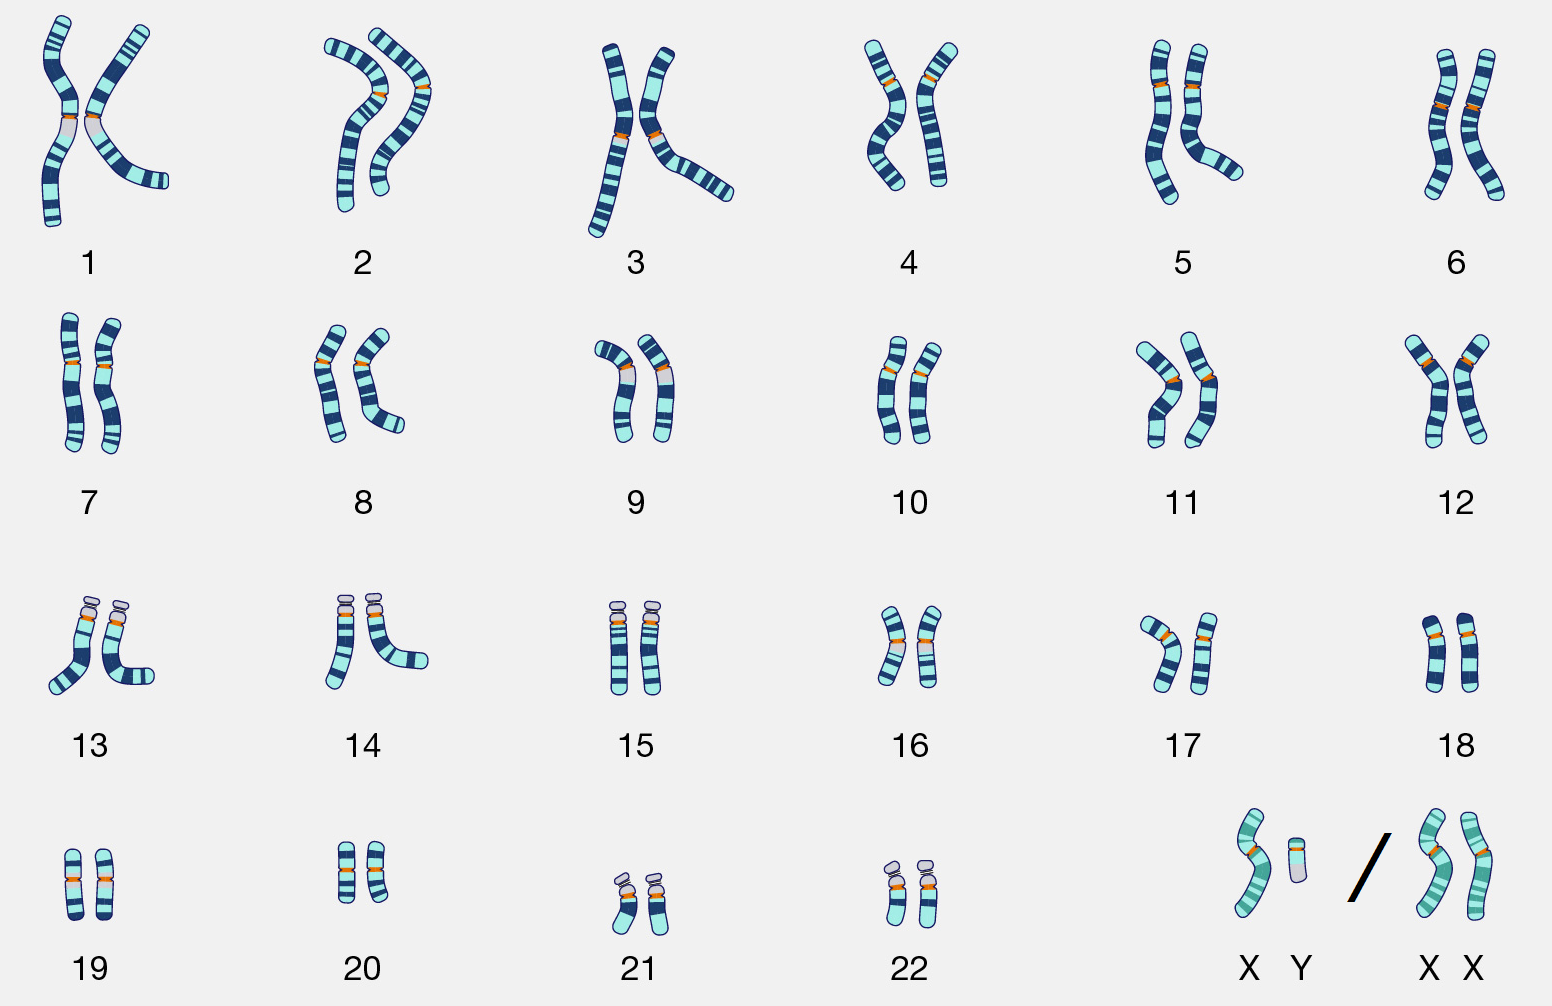
\includegraphics[width=1\linewidth]{image004}
		\caption{\small\textit{\color{timhieukhoahoc}Hình $3$. Ở người có tổng cộng $46$ nhiễm sắc thể chia làm $23$ cặp. $22$ cặp đầu là các cặp tương đồng, mỗi gen đều có một bản sao ở cùng vị trí trên mỗi nhiễm sắc thể trong cặp. Cặp cuối cùng là cặp nhiễm sắc thể giới tính.}}
		\vspace*{-10pt}
	\end{figure}
	Các nhiễm sắc thể thường đi theo cặp. Hai nhiễm sắc thể cùng một cặp có cấu trúc giống nhau. Mỗi vị trí tương ứng của hai nhiễm sắc thể này sẽ mã hóa cùng một gen. Do đó mỗi gen trong cơ thể sinh vật sẽ có $2$ phiên bản (gọi là allele) ở cặp nhiễm sắc thể chứa nó. Khi hai allele giống nhau (ví dụ $AA$ hoặc $aa$) thì gọi là đồng hợp tử; còn nếu chúng là dạng lai ($Aa$) thì gọi là dị hợp tử.
	\vskip 0.1cm 
	Do kết quả của quá trình giảm phân, chỉ có một trong hai allele của gen được sao chép lại vào tế bào sinh sản. Sự kết hợp của hai allele, một từ bố và một từ mẹ, tạo ra trạng thái di truyền (gọi là kiểu gen) của thế hệ sau. Đặc điểm biểu hiện ra ngoài trong thực tế (kiểu hình) sẽ phụ thuộc vào tính trội/lặn của các allele. Dựa trên nguyên lý này, ta có thể giải thích các thí nghiệm của Mendel như trong Hình $4$ và Hình $5$.  
	\begin{figure}[H]
		\centering
		%		\vspace*{-5pt}
		\captionsetup{labelformat= empty, justification=centering}
		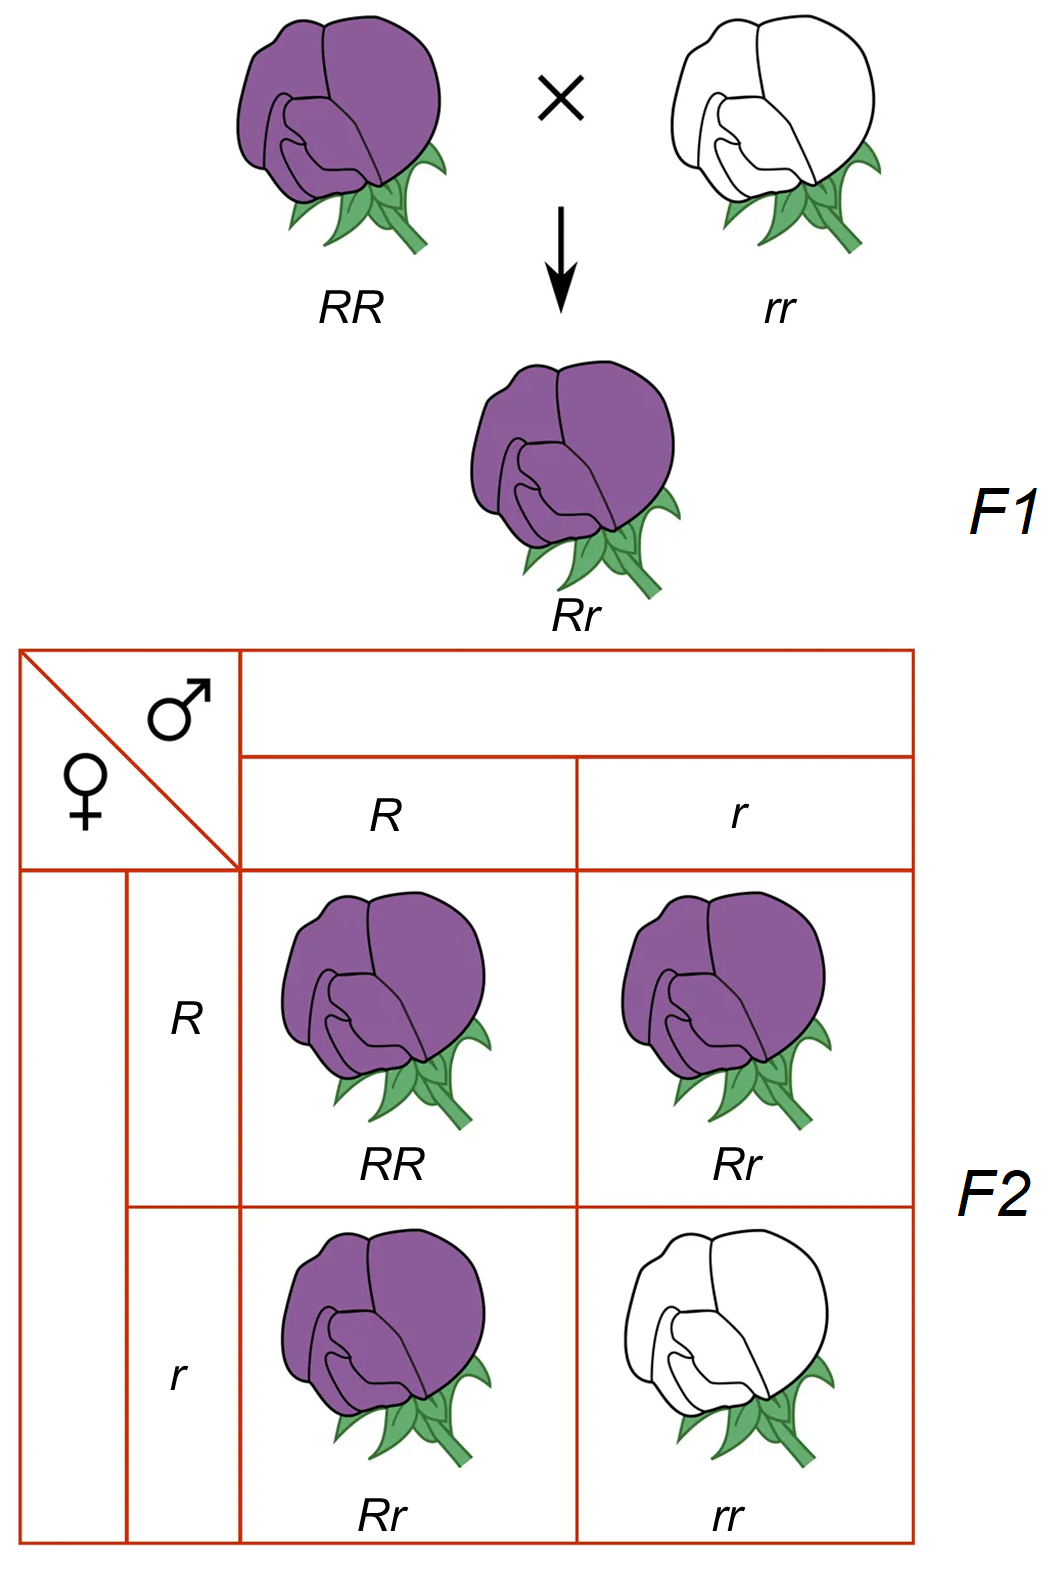
\includegraphics[width=0.98\linewidth]{image005}
		\caption{\small\textit{\color{timhieukhoahoc}Hình $4$. Lai một cặp tính trạng giữa cây thuần hoa tím ($RR$) và cây thuần hoa trắng ($rr$). Hoa tím là trội so với hoa trắng. F$1$ nhận một nửa từ mỗi bố mẹ nên có kiểu gen là $Rr$ và biểu hiện là hoa tím (do $R$ là trội so với $r$). Khi F$1$ tự thụ phấn cho ra F$2$, mỗi loại tế bào sinh sản đực/cái của F$1$ đều có hai kiểu gen $R$ và $r$ với khả năng như nhau, cho ta tổ hợp ở F$2$ như trong hình với tỷ lệ $RR : Rr : rr$ là $1 : 2 :1$ và tỷ lệ hoa tím : hoa trắng là $3$~:~$1$.}}
		\vspace*{-10pt}
	\end{figure}
	Trong trường hợp Hình $5$, ta thừa nhận rằng quá trình tạo tổ hợp của mỗi gen là độc lập với nhau. Khi hai gen nằm ở các cặp nhiễm sắc thể khác nhau, việc này là hiển nhiên. Tuy nhiên, với hai gen nằm trên cùng một cặp nhiễm sắc thể, liệu tỷ lệ cho các tổ hợp của Mendel vẫn còn đúng không?
	\vskip 0.1cm
	Câu trả lời liên quan đến hiện tượng trao đổi chéo (cross over) trong quá trình giảm phân tạo tế bào sinh sản. Quá trình này được Thomas Morgan và sinh viên Alfred Sturtevant của ông phát hiện từ các thí nghiệm trên ruồi giấm. Trong quá trình giảm phân từ một tế bào ban đầu tạo thành bốn tế bào sinh sản (gọi là gamete), có thể xảy ra sự hoán vị một số đoạn giữa các nhiễm sắc thể (Hình $6$). Do đó dù mỗi gamete chỉ có một nhiễm sắc thể đơn, nó có thể không hoàn toàn giống với một trong hai nhiễm sắc thể của cặp ban đầu mà là một tổ hợp từ chúng. Do việc hoán vị của quá trình trao đổi chéo này là ngẫu nhiên nên với những gen trên cùng nhiễm sắc thể, nếu chúng cách nhau đủ xa thì quá trình tổ hợp của chúng vẫn độc lập với nhau theo định luật Mendel.  
	\begin{figure}[H]
		\centering
		\vspace*{-5pt}
		\captionsetup{labelformat= empty, justification=centering}
		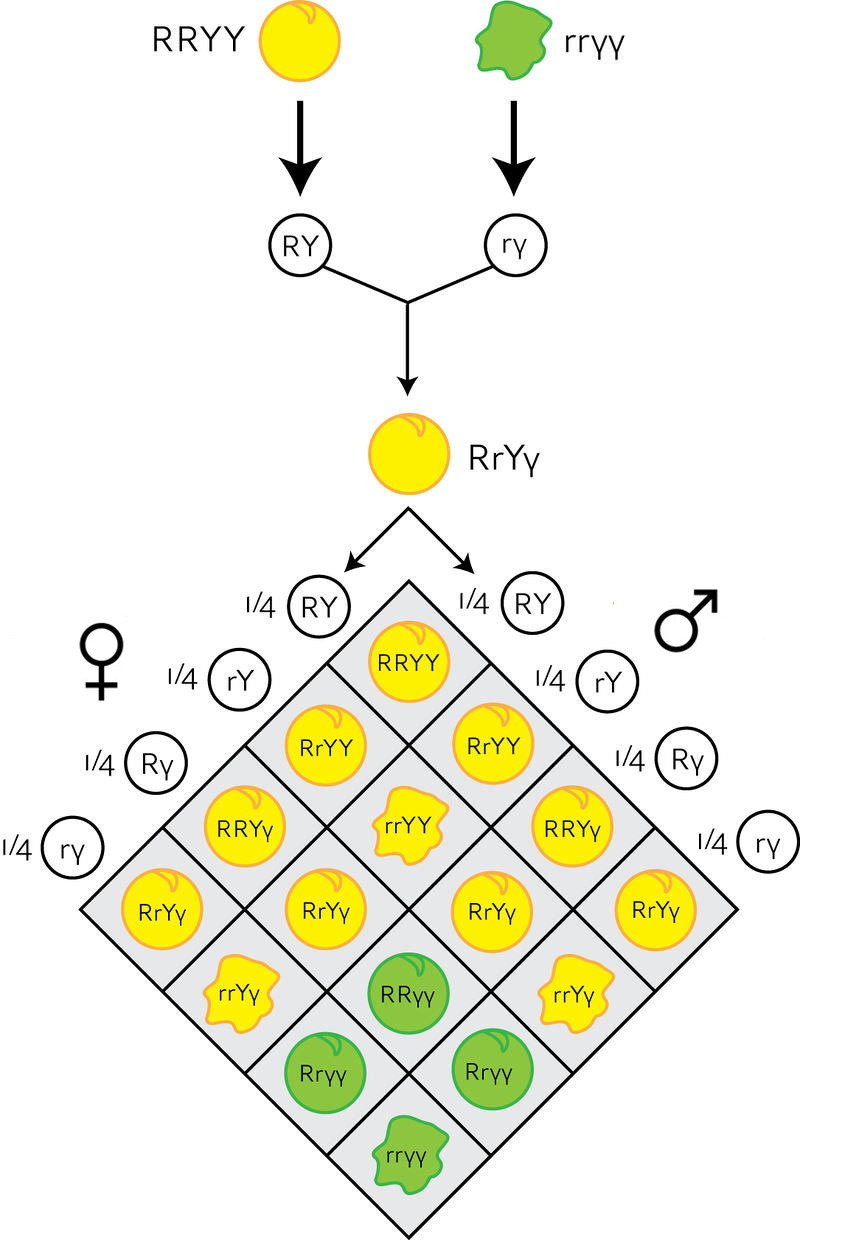
\includegraphics[width=0.98\linewidth]{image006}
		\caption{\small\textit{\color{timhieukhoahoc}Hình $5$. Lai hai cặp tính trạng: $R$ (hạt trơn -- trội), $r$ (hạt nhăn -- lặn) và $Y$ (hạt vàng -- trội), $y$ (hạt xanh -- lặn). Do mỗi cặp tính trạng di truyền độc lập nên F$1$ sẽ có kiểu gen $RrYy$ và các tế bào sinh sản của F$1$ có xác suất bằng nhau ($1/4$) cho mỗi kiểu gen ($RY, Ry, rY, ry$). Do công thức nhân xác suất, mỗi ô trong bảng có xác suất $1/16$. Tỷ lệ kiểu hình thu được là $9 : 3 : 3 : 1$ cho vàng trơn~:~vàng nhăn~:~xanh trơn~:~xanh nhăn. Dạng bảng như trên còn được gọi là bảng Punnet theo tên nhà di truyền học Reginald Punnet, đồng tác giả cuốn sách của William Bateson về di truyền học Mendel.}}
		\vspace*{-5pt}
	\end{figure}
	\begin{figure}[H]
		\centering
		%		\vspace*{-5pt}
		\captionsetup{labelformat= empty, justification=centering}
		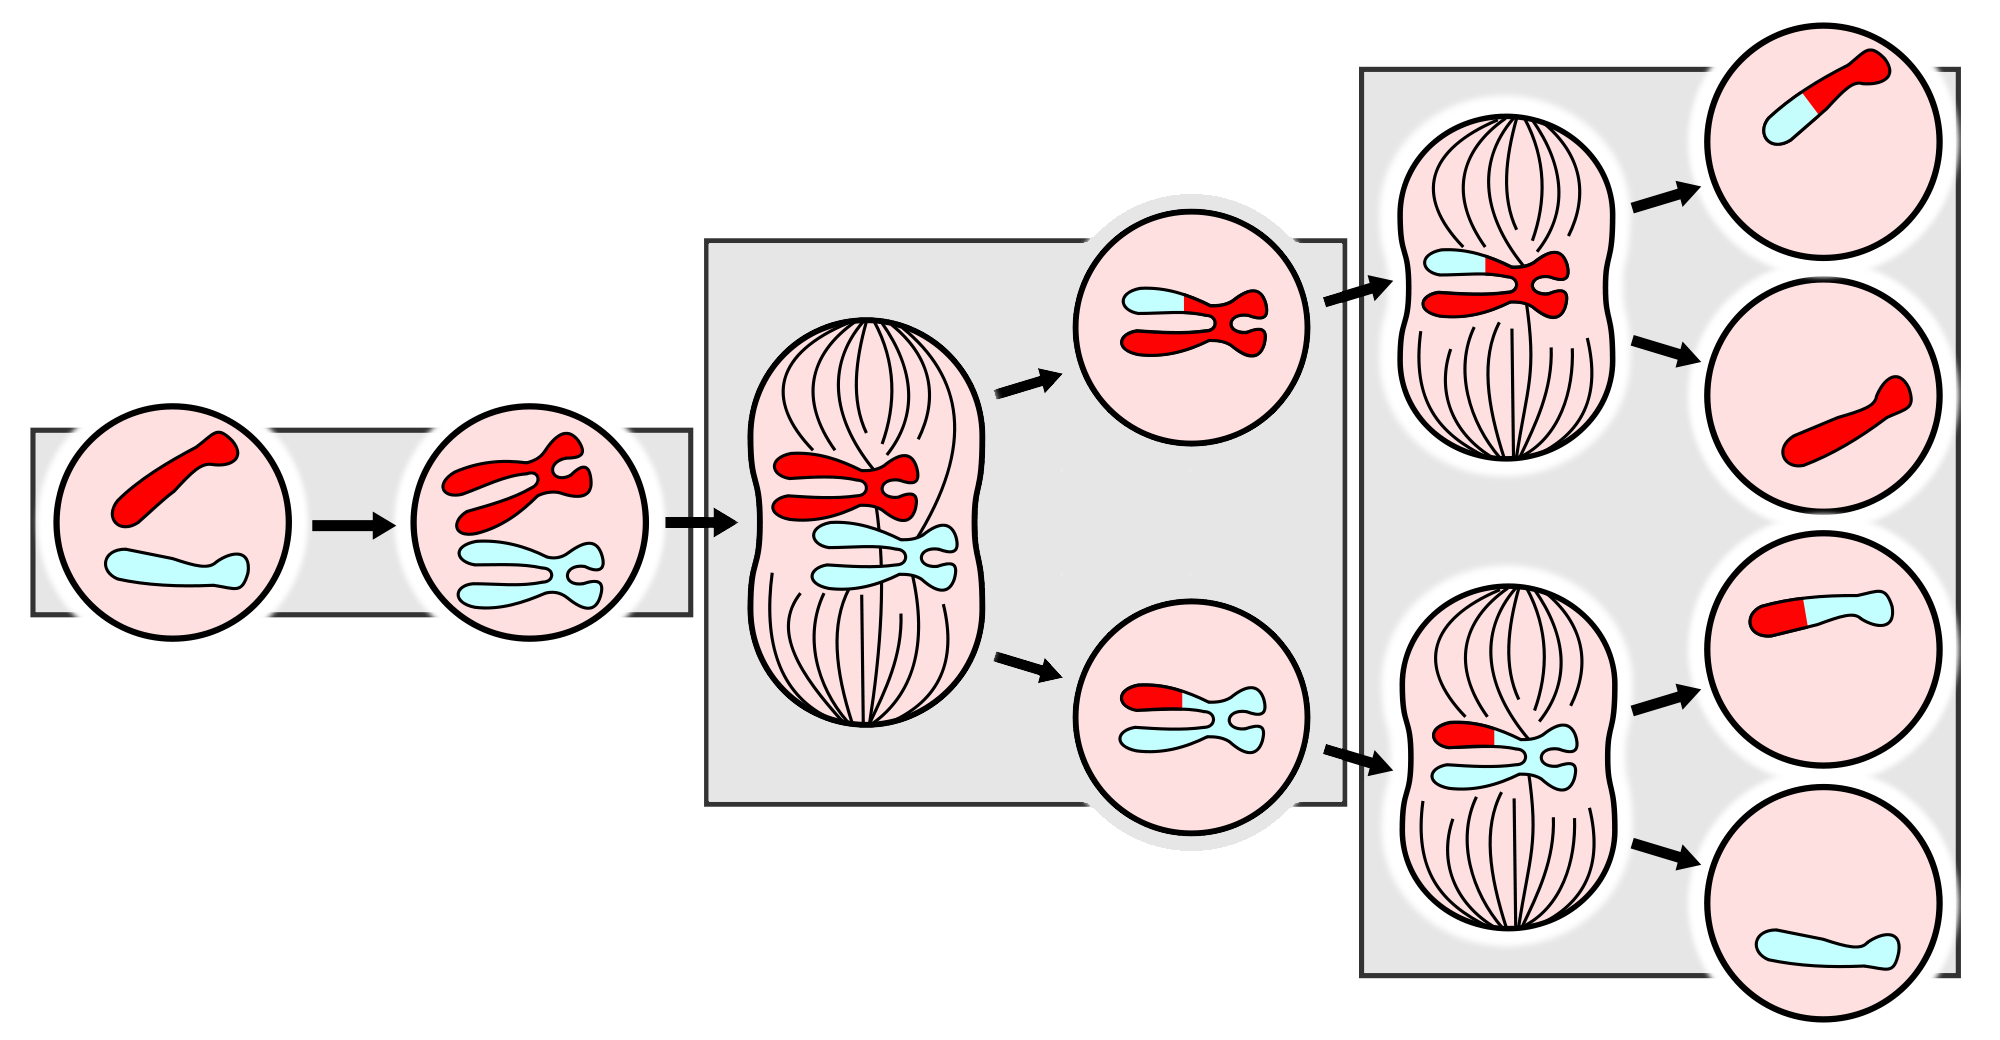
\includegraphics[width=1\linewidth]{image007}
		\caption{\small\textit{\color{timhieukhoahoc}Hình $6$. Minh họa quá trình giảm phân có trao đổi chéo. Hai nhiễm sắc thể ban đầu của cặp tương đồng được sao chép gấp đôi. Trao đổi chéo diễn ra giữa hai nhiễm sắc thể không có cùng bản gốc. Sau đó, do phân chia tế bào, bốn nhiễm sắc thể đơn trở thành vật liệu di truyền của bốn tế bào sinh sản.}}
		\vspace*{-10pt}
	\end{figure}
	Trong trường hợp hai gen đủ gần, do hoán vị chỉ xảy ra khi điểm trao đổi chéo nằm ở giữa vị trí của hai gen nên xác suất của việc xảy ra hoán vị trong trường hợp này nhỏ hơn nhiều. Tần số xảy ra trao đổi chéo sẽ tăng theo khoảng cách giữa hai gen. Trong thực nghiệm, tần số này có thể được xác định thông qua lai tạo (Hình $8$).
	\begin{figure}[H]
		\centering
		\vspace*{-5pt}
		\captionsetup{labelformat= empty, justification=centering}
		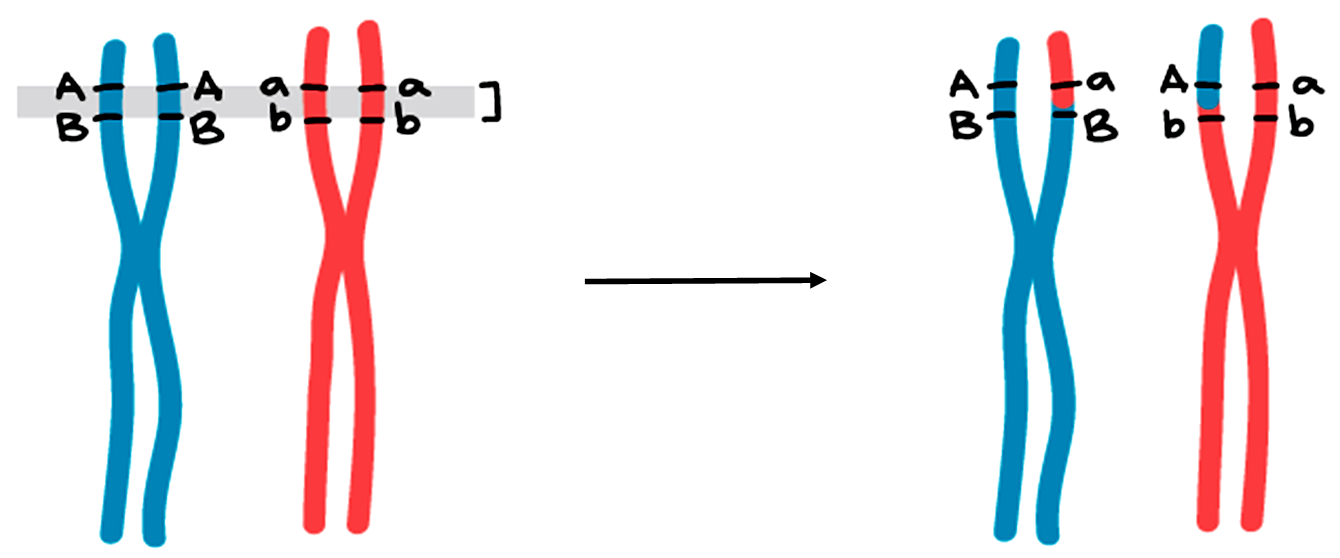
\includegraphics[width=1\linewidth]{image008}
		\caption{\small\textit{\color{timhieukhoahoc}Hình $7$. Quá trình tái tổ hợp do hoán vị chỉ xảy ra nếu vị trí trao đổi chéo nằm giữa vị trí của hai gen. Do đó nếu hai gen ở gần nhau thì quá trình này có xác suất thấp.}}
		\vspace*{-10pt}
	\end{figure}
	Tỷ lệ phần trăm các cá thể F$2$ dạng tái tổ hợp (khác cả ông lẫn bà) so với tổng số cá thể F$2$ được dùng để đại diện cho khoảng cách giữa hai gen. Đơn vị của khoảng cách này là centimorgan (đặt theo tên của Thomas Morgan), cứ $1\%$ là $1$ centimorgan. Giá trị lớn nhất của khoảng cách sẽ là $50$ centimorgan, ứng với trường hợp các tổ hợp tuân theo định luật Mendel (tỷ lệ giữa $4$ tổ hợp sẽ là $1 : 1 : 1 : 1$).
	\begin{figure}[H]
		\centering
		%		\vspace*{-5pt}
		\captionsetup{labelformat= empty, justification=centering}
		$a)$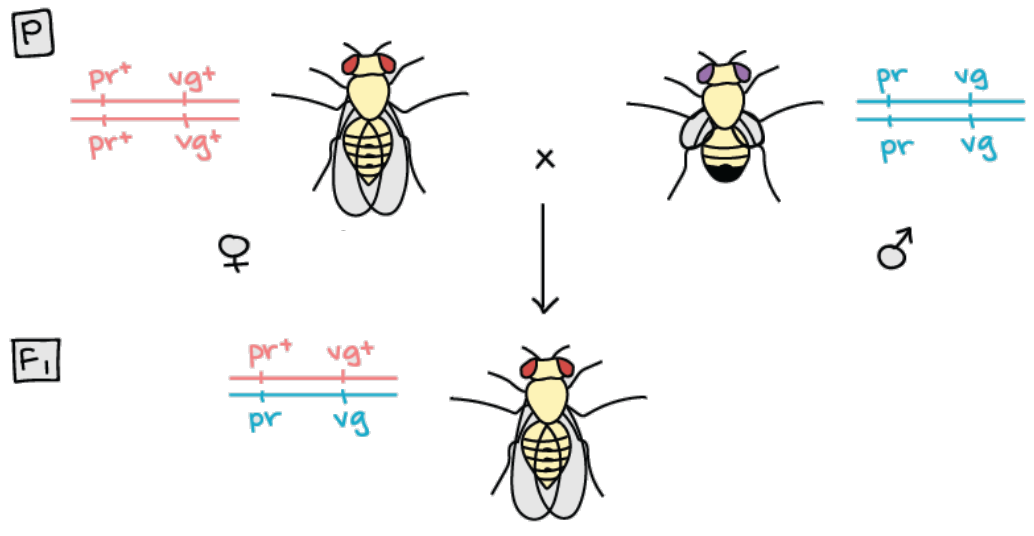
\includegraphics[width=0.95\linewidth]{image009}
		$b)$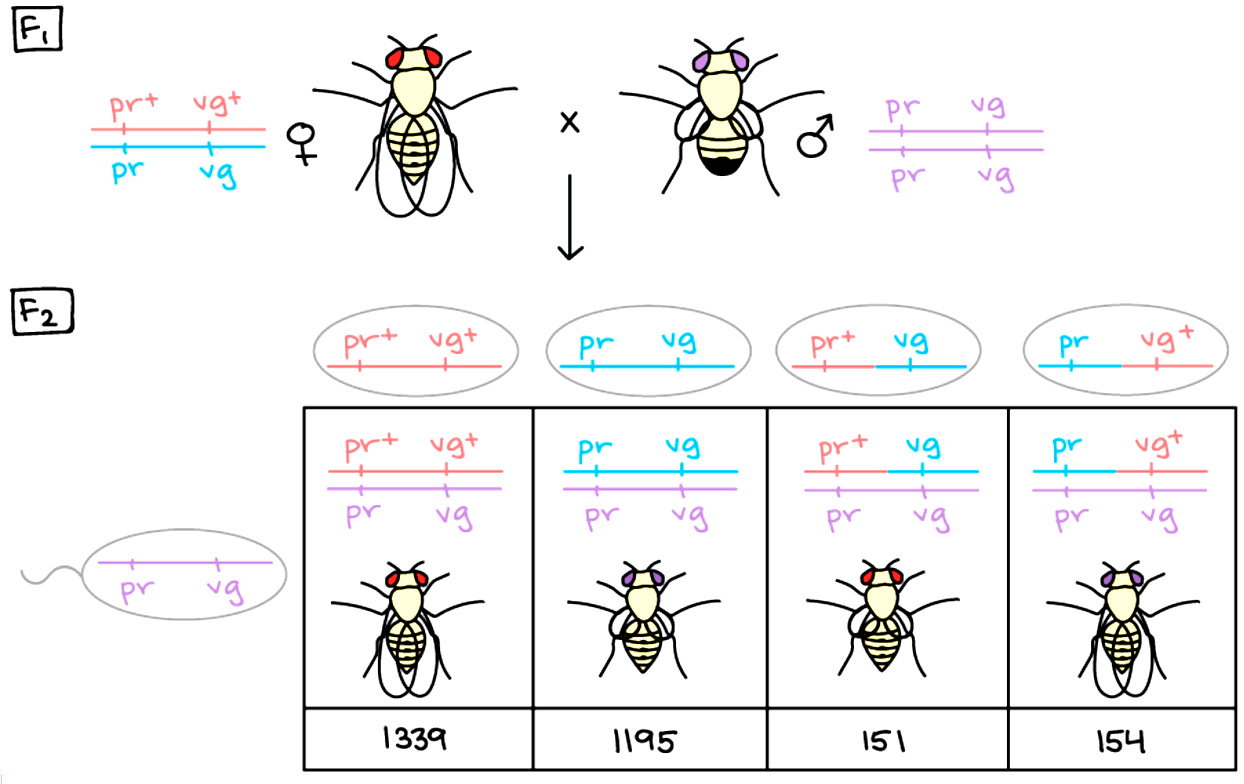
\includegraphics[width=0.95\linewidth]{image010}
		\caption{\small\textit{\color{timhieukhoahoc}Hình $8$. Thí nghiệm đo khoảng cách gen ở ruồi giấm. Có hai cặp tính trạng: $pr+$ (mắt đỏ -- trội), $pr$ (mắt tím -- lặn) và $vg+$ (cánh dài -- trội), $vg$ (cánh ngắn -- lặn). $a)$ Các cá thể cái trội hoàn toàn (mắt đỏ cánh dài) lai với các cả thể lặn hoàn toàn (mắt tím cánh ngắn). Do các kiểu gen đều là đồng hợp tử nên hai gen của F$1$ có dạng trên cặp nhiễm sắc thể như trong hình. $b)$ Các con cái từ F$1$ được lai với cá thể đực có kiểu gen lặn giống bố của F$1$. Các cá thể F$2$ từ các trứng có các tổ hợp của F$1$ không phải do hoán vị sẽ giống ông hoặc bà của nó (mắt đỏ cánh dài hoặc mắt tím cánh ngắn) còn các cá thể F$2$ từ các trứng có các tổ hợp của F$1$ tạo thành bởi hoán vị do tái tổ hợp sẽ có kiểu hình lẫn lộn (mắt đỏ cánh ngắn hoặc mắt tím cánh dài). Ví dụ trong hình, khoảng cách gen có thể được tính theo: $(151 + 154)/(1339 + 1195 + 151 +154) = 10,7$\% hay $10,7$ centimorgan.}}
		\vspace*{-10pt}
	\end{figure}
	%	\vskip 0.1cm
	Tuy khoảng cách đo bằng xác suất thực nghiệm này không tỷ lệ trực tiếp với khoảng cách vật lý giữa hai gen trên nhiễm sắc thể, nó vẫn có giá trị trong việc sắp xếp thứ tự giữa các gen. Dựa trên khoảng cách của từng cặp gen, người ta có thể tiến hành xây dựng được bản đồ gen của sinh vật thông qua các thí nghiệm di truyền. Alfred Sturtevant đã thành lập bản đồ gen đầu tiên cho một nhiễm sắc thể của ruồi giấm dựa theo phương pháp này.
	\vskip 0.1cm
	Ngày nay với các công nghệ giải trình tự thế hệ mới cho phép biết trình tự chính xác của các DNA trên nhiễm sắc thể thì việc lập bản đồ gen cũng trở nên dễ dàng hơn nhiều.
	\vskip 0.1cm
	$\pmb{5.}$ \textbf{\color{timhieukhoahoc}Lời kết}
	\vskip 0.1cm
	Trong giai đoạn sau bài báo năm $1866$, Mendel vẫn tiếp túc nghiên cứu di truyền học. Trong các bức thư trao đổi với nhà sinh học von Nageli, ông trình bày các phân tích của mình, đặc biệt liên quan đến các công bố của Darwin. Nhiều quan điểm trong số đó đã gần với những gì chúng ta biết ngày nay. Tuy nhiên, Mendel không công bố công trình khoa học nào từ những nhận định này. Công việc ở tu viện sau khi nhậm chức quản lý ở đây năm $1868$ cũng chiếm hết thời gian của ông. Theo lời kể của người cháu họ thì, do có nhiều kẻ thù trong nhà thờ do các nghiên cứu sinh học, Mendel có các tài liệu khoa học được chuẩn bị để công bố sau khi ông mất. Tuy nhiên, cuối cùng thì gia đình ông cũng không nhận được gì từ phía giáo hội.
	\vskip 0.1cm
	Ngày nay, vai trò của Mendel trong di truyền học cũng như khía cạnh lịch sử liên quan đến khám phá của ông vẫn là một đề tài được nhiều nhà nghiên cứu quan tâm từ hơn một thế kỷ qua. Có thể nói, Mendel vẫn luôn là một tấm gương về sự miệt mài cần mẫn đi kèm với tính sáng tạo và cái nhìn khách quan trong nghiên cứu khoa học.
	\begin{figure}[H]
		\centering
		\vspace*{-5pt}
		\captionsetup{labelformat= empty, justification=centering}
		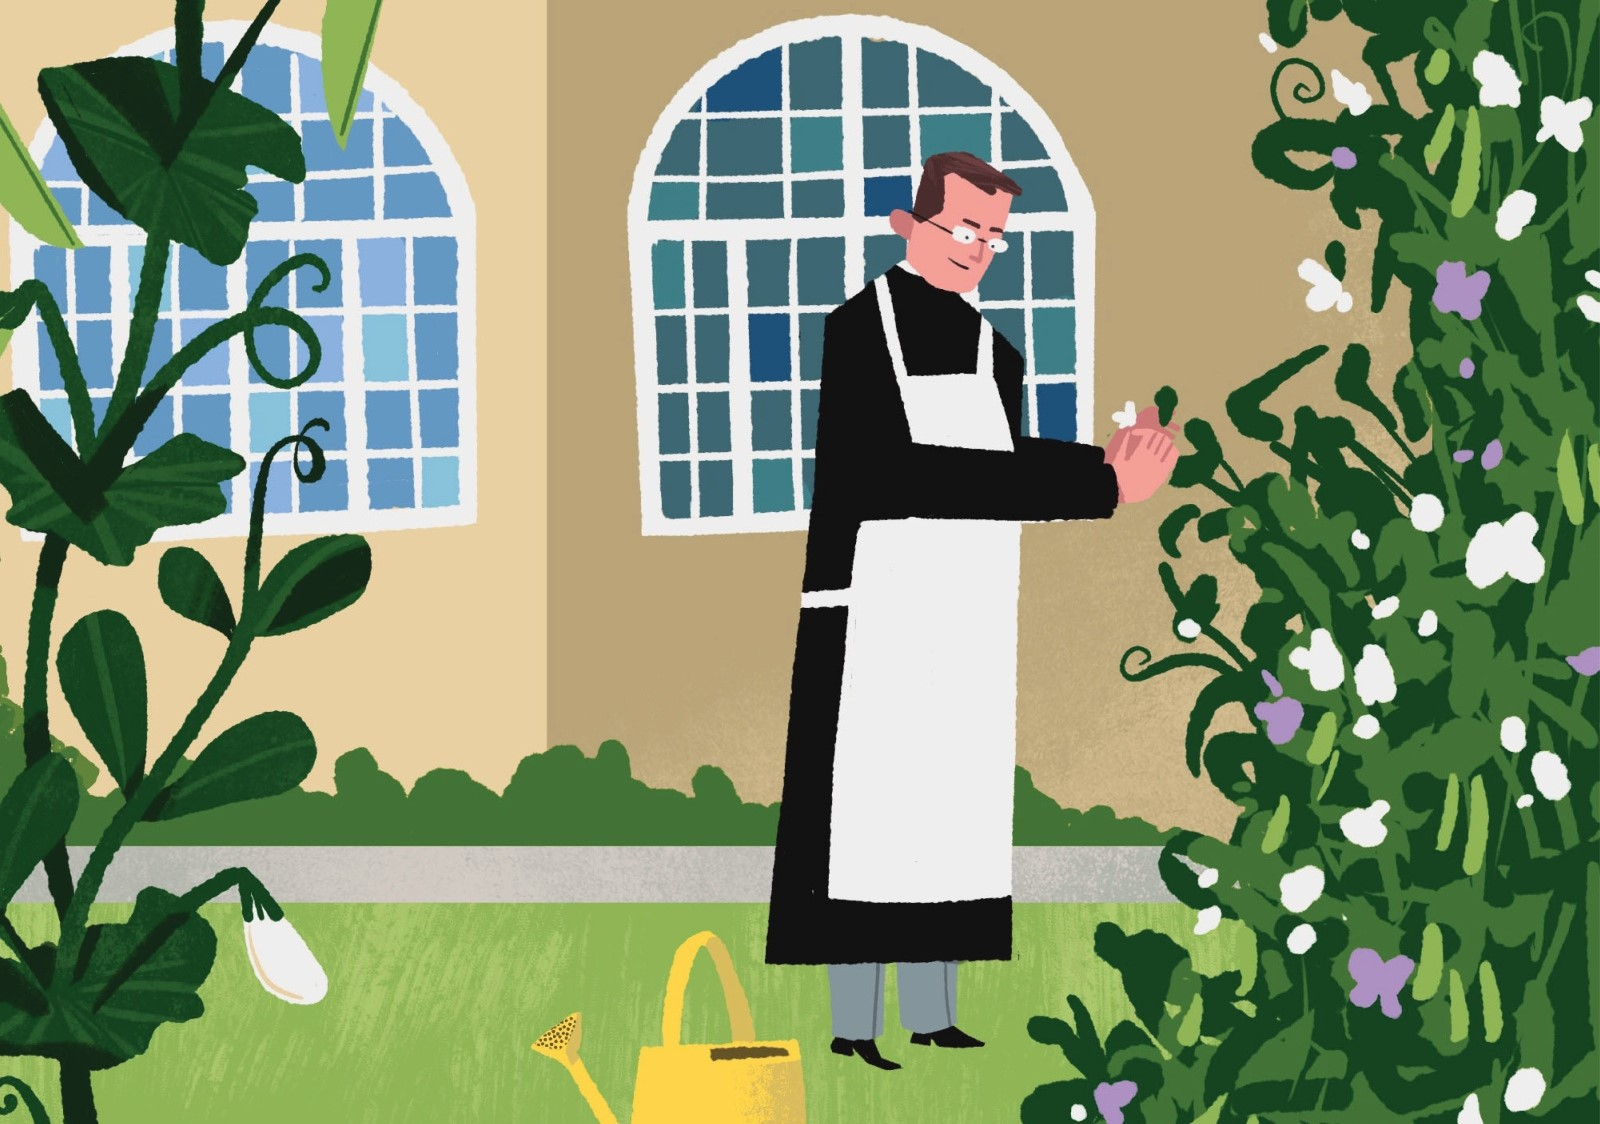
\includegraphics[width=1\linewidth]{image011}
		\vspace*{-10pt}
	\end{figure}
	\columnbreak
	\textbf{\color{timhieukhoahoc}Tài liệu tham khảo}
	\vskip 0.1cm
	[$1$] Bizzo, N. and El--Hani, C.N. ($2009$). Darwin and Mendel: evolution and genetics. \textit{Journal of Biological Education}, $43(3)$, pp.$108-114$. doi:$10.1080$/$00219266$.$2009$.\\$9656164$.
	\vskip 0.1cm
	[$2$] Fairbanks, D.J. ($2019$). Mendel and Darwin: untangling a persistent enigma. \textit{Heredity}, $124(2)$, pp.$263-273$. doi:$10.1038$/s$41437$--$019$--$0289$--$9$.
	\vskip 0.1cm
	[$3$] Franklin, A. and Al, E. ($2008$). \textit{Ending the Mendel--Fisher controversy}. Pittsburgh Pa: University Of Pittsburgh Press.
	\vskip 0.1cm
	[$4$] Gayon, J. ($2016$). From Mendel to epigenetics: History of genetics. \textit{Comptes Rendus Biologies}, $339(7-8)$, pp.$225-230$. doi:$10$.$1016$/j.crvi.$2016$.$05$.$009$.
	\vskip 0.1cm
	[$5$] Klein, J. and Klein, N. ($2013$). \textit{Solitude of a Humble Genius -- Gregor Johann Mendel: Volume} $1$. Berlin, Heidelberg Springer Berlin Heidelberg.
\end{multicols}